\section{Enumeração Exaustiva}
\subsection{Exemplo}


\begin{frame}
	\only<1-2>
	{
		\begin{columns}
			\begin{column}{0.7\textwidth}
				\centering
				\begin{exampleblock}{Exemplo 1 - Modelo Matemático Completo}
					\scriptsize
					\begin{table}
						\begin{tabular}{r c l}
							$ \max Z = 600x_1+800x_2$ & 
\includegraphics[width=0.8cm,height=0.2cm]{seta2.png} & Função Objetivo \\
							sujeito a & & \\
							$x_1+x_2 \le 100$ & 
\includegraphics[width=0.8cm,height=0.2cm]{seta2.png}& Área Cultivo \\
							$3x_1+2x_2 \le 240$ & 
\includegraphics[width=0.8cm,height=0.2cm]{seta2.png}& Mão de Obra \\
							$x_1 \le 60 $ & 
\includegraphics[width=0.8cm,height=0.2cm]{seta2.png}& Produção Cereal \textbf{A} \\
							$x_2 \le 80 $ &
\includegraphics[width=0.8cm,height=0.2cm]{seta2.png} & Produção Cereal \textbf{B} \\
							$x_1, x_2 \ge 0$ & 
\includegraphics[width=0.8cm,height=0.2cm]{seta2.png}& Produção \\
						\end{tabular}
					\end{table}
				\end{exampleblock}
			\end{column}
			\begin{column}{0.3\textwidth}
				\centering
				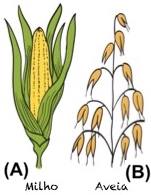
\includegraphics[width=2cm,height=3cm]{milho_aveia2.png}
			\end{column}
		\end{columns}
	}
	\only<3>
	{
		\centering
		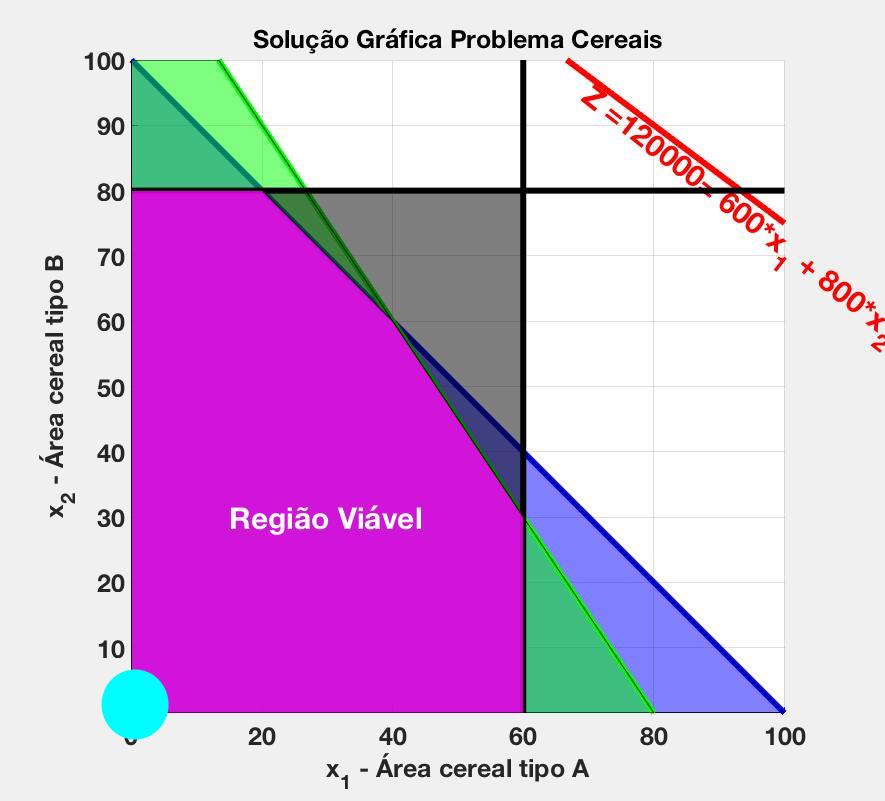
\includegraphics[width=4.2cm,height=4.2cm]{Exaustiva_2.jpeg}
	}
	\only<4>
	{
		\centering
		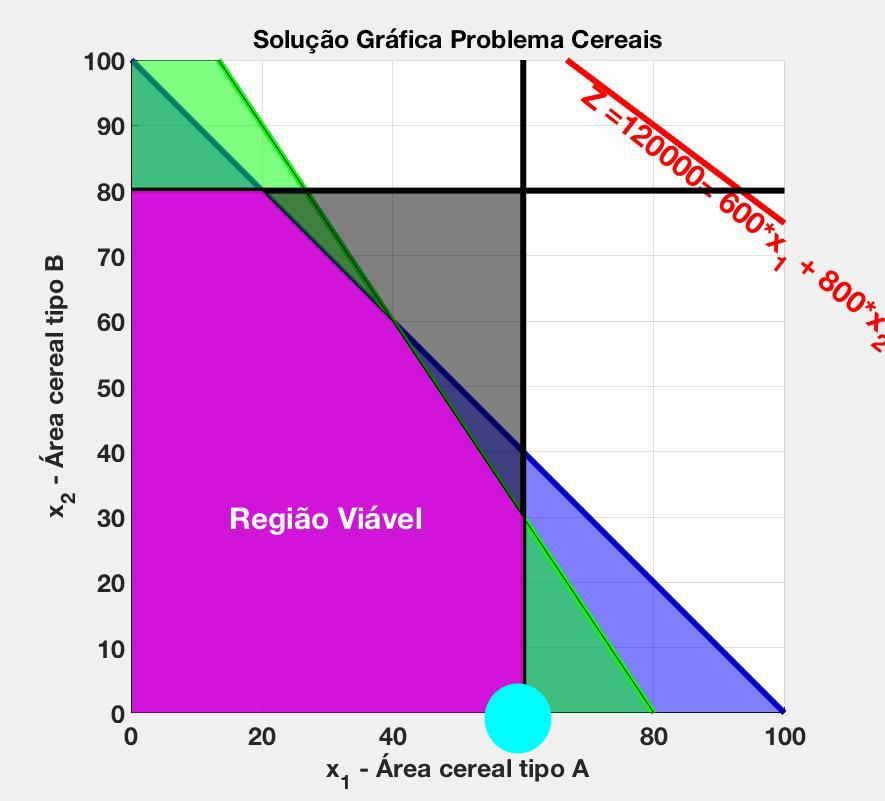
\includegraphics[width=4.2cm,height=4.2cm]{Exaustiva_3.jpeg}
	}
	\only<5>
	{
		\centering
		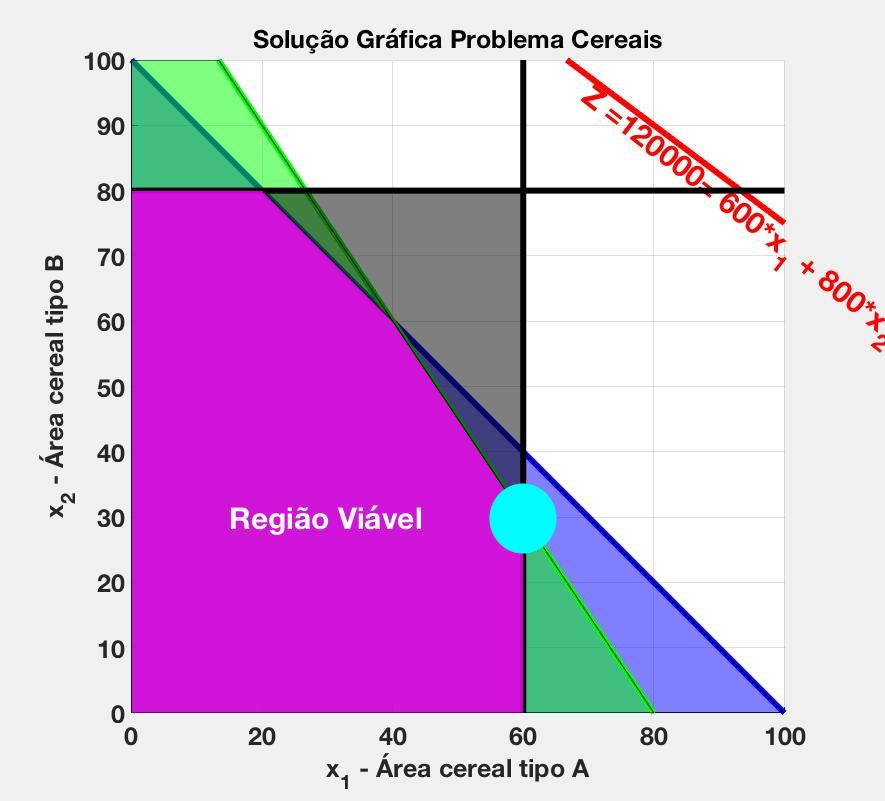
\includegraphics[width=4.2cm,height=4.2cm]{Exaustiva_4.jpeg}
	}
	\only<6>
	{
		\centering
		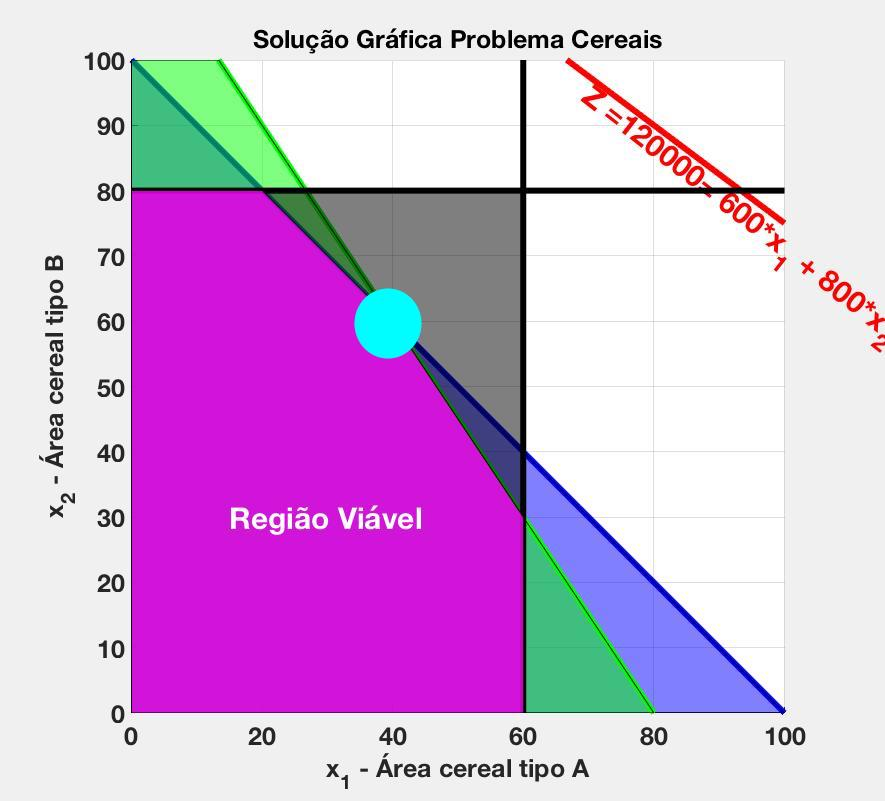
\includegraphics[width=4.2cm,height=4.2cm]{Exaustiva_5.jpeg}
	}
	\only<7>
	{
		\centering
		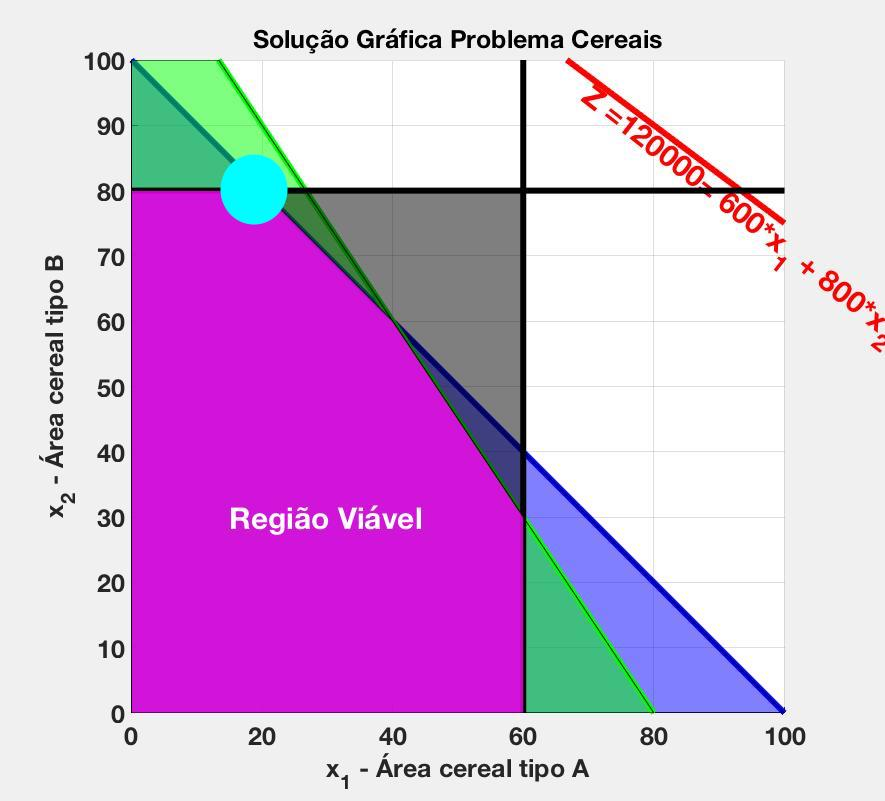
\includegraphics[width=4.2cm,height=4.2cm]{Exaustiva_6.jpeg}
	}
	\only<8>
	{
		\centering
		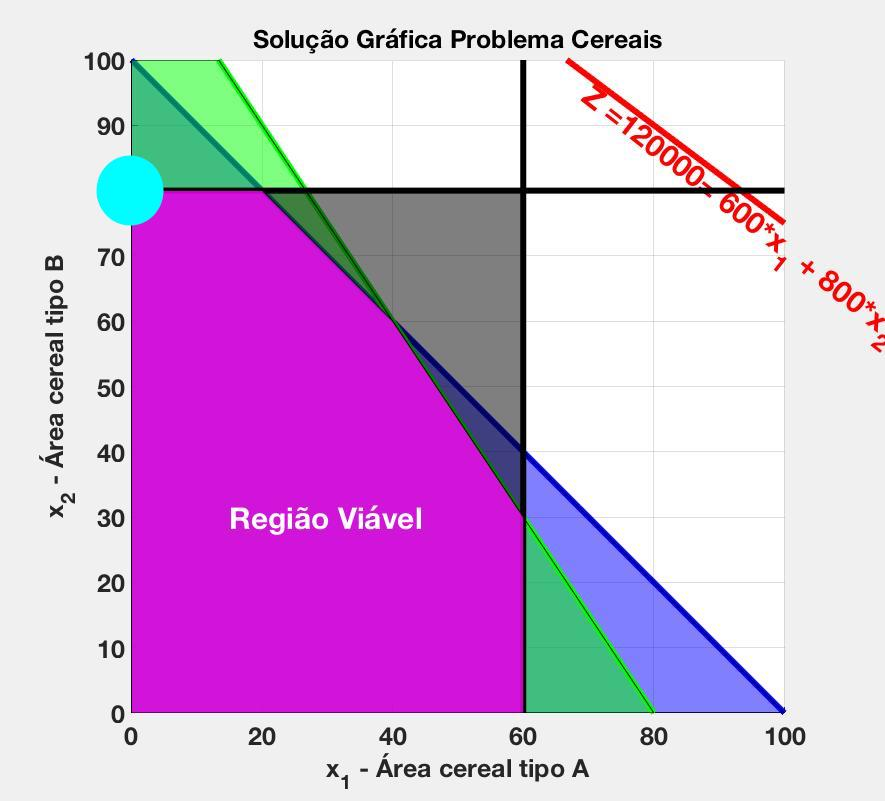
\includegraphics[width=4.2cm,height=4.2cm]{Exaustiva_7.jpeg}
	}
	\only<9->
	{
		\centering
		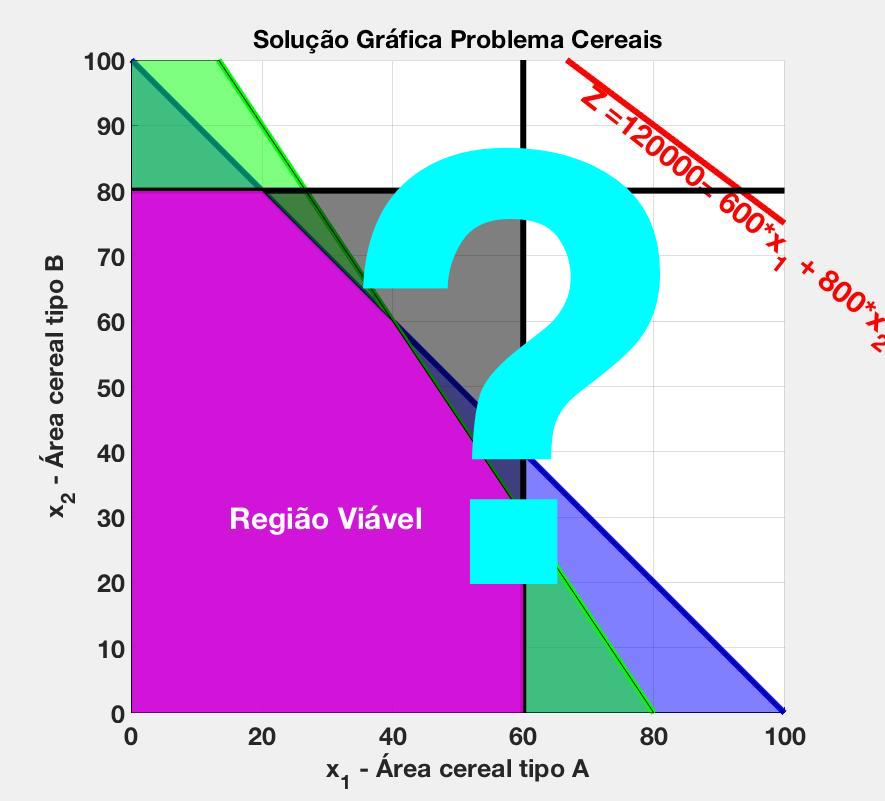
\includegraphics[width=4.2cm,height=4.2cm]{Exaustiva_1.jpeg}
	}

	\only<2-3>
	{
		\begin{block}{Forma Padrão - {\color{cyan}Escolha 1}}
			\begin{columns}
				\begin{column}{0.35\textwidth}
					$
						\begin{matrix}
							\max Z - 600x_1 - 800x_2 = 0 \\
						\end{matrix}
					$ \\
					\text{Sujeito a:} \\
					$
						\begin{matrix}
							x_1+x_2  {+\color{red}x_3} = 100 \\
							3x_1+2x_2 {+ \color{red}x_4} = 240 \\
							x_1  {+ \color{red}x_5} = 60 \\
							x_2 {+ \color{red}x_6} = 80 \\
							x_1,x_2, {\color{red} x_3, x_4, x_5, x_6} \ge 0 \\
						\end{matrix}
					$
				\end{column}
				\vline
				\hspace{0.1cm}
				\begin{column}{0.45\textwidth}
					$
						\begin{matrix}
							\text{VB} \left\{  \begin{matrix}
														 x_3 = 100 \\
														 x_4 = 240 \\
														 x_5 = 60 \\
														 x_6 = 80 \\
								   \end{matrix} 
						   \right.
							&
							\text{VNB} \left\{  \begin{matrix}
														 x_1 = 0 \\
														 x_2 = 0 \\
								   \end{matrix} 
						   \right. 
							\\
							 & \\
						\end{matrix}
					$
					$ {\color{red}Z = 0} $
				\end{column}
			\end{columns}
		\end{block}
	}
	\only<4>
	{
		\begin{block}{Forma Padrão - {\color{cyan}Escolha 2}}
			\begin{columns}
				\begin{column}{0.35\textwidth}
					$
						\begin{matrix}
							\max Z - 600x_1 - 800x_2 = 0 \\
						\end{matrix}
					$ \\
					\text{Sujeito a:} \\
					$
						\begin{matrix}
							x_1  + {\color{red}\cancel{x_2}}  + x_3                   = 100 \\
							3x_1 + 2{\color{red}\cancel{x_2}}       + x_4             = 240 \\
							x_1                     + {\color{red}\cancel{x_5}}       = 60 \\
							{\color{red}\cancel{x_2}}                           + x_6 = 80 \\
							x_1,x_2, x_3, x_4, x_5, x_6 \ge 0 \\
						\end{matrix}
					$
				\end{column}
				\vline
				\hspace{0.1cm}
				\begin{column}{0.45\textwidth}
						$
							\begin{matrix}
								\text{VB} \left\{  \begin{matrix}
																 x_1 = 60 \\
																 x_3 = 40 \\
																 x_4 = 60 \\
																 x_6 = 80 \\
												   \end{matrix} 
										   \right.
								&
								\text{VNB} \left\{  \begin{matrix}
																 x_2 = 0 \\
																 x_5 = 0 \\
												   \end{matrix} 
										   \right. 
								\\
							 & \\
							\end{matrix}							
						$
						{\color{red}$ Z = 36000 $}
				\end{column}
			\end{columns}
		\end{block}
	}
	\only<5>
	{
		\begin{block}{Forma Padrão - {\color{cyan}Escolha 3}}
			\begin{columns}
				\begin{column}{0.35\textwidth}
					$
						\begin{matrix}
							\max Z - 600x_1 - 800x_2 = 0 \\
						\end{matrix}
					$ \\
					\text{Sujeito a:} \\
					$
						\begin{matrix}
							x_1  + x_2  + x_3                   = 100 \\
							3x_1 + 2x_2       + {\color{red}\cancel{x_4}}             = 240 \\
							x_1                     + {\color{red}\cancel{x_5}}       = 60 \\
							x_2                           + x_6 = 80 \\
							x_1,x_2, x_3, x_4, x_5, x_6 \ge 0 \\
						\end{matrix}
					$
				\end{column}
				\vline
				\hspace{0.1cm}
				\begin{column}{0.45\textwidth}
						$
							\begin{matrix}
								\text{VB} \left\{  \begin{matrix}
																 x_1 = 60 \\
																 x_2 = 30 \\
																 x_3 = 10 \\
																 x_6 = 50 \\
												   \end{matrix} 
										   \right.
								&
								\text{VNB} \left\{  \begin{matrix}
																 x_4 = 0 \\
																 x_5 = 0 \\
												   \end{matrix} 
										   \right. 
								\\
							 & \\
							\end{matrix}
						$
						{\color{red}$ Z = 60000 $}
				\end{column}
			\end{columns}
		\end{block}
	}
	\only<6>
	{
		\begin{block}{Forma Padrão - {\color{cyan}Escolha 4}}
			\begin{columns}
				\begin{column}{0.35\textwidth}
					$
						\begin{matrix}
							\max Z - 600x_1 - 800x_2 = 0 \\
						\end{matrix}
					$ \\
					\text{Sujeito a:} \\
					$
						\begin{matrix}
							x_1  + x_2  + {\color{red}\cancel{x_3}}                   = 100 \\
							3x_1 + 2x_2       + {\color{red}\cancel{x_4}}             = 240 \\
							x_1                     + x_5       = 60 \\
							x_2                           + x_6 = 80 \\
							x_1,x_2, x_3, x_4, x_5, x_6 \ge 0 \\
						\end{matrix}
					$
				\end{column}
				\vline
				\hspace{0.1cm}
				\begin{column}{0.45\textwidth}
						$
							\begin{matrix}
								\text{VB} \left\{  \begin{matrix}
																 x_1 = 40 \\
																 x_2 = 60 \\
																 x_5 = 20 \\
																 x_6 = 20 \\
												   \end{matrix} 
										   \right.
								&
								\text{VNB} \left\{  \begin{matrix}
																 x_3 = 0 \\
																 x_4 = 0 \\
												   \end{matrix} 
										   \right. 
								\\
							 & \\
							\end{matrix}
						$
						{\color{red}$ Z = 72000 $}
				\end{column}
			\end{columns}
		\end{block}
	}
	\only<7>
	{
		\begin{block}{Forma Padrão - {\color{cyan}Escolha 5}}
			\begin{columns}
				\begin{column}{0.35\textwidth}
					$
						\begin{matrix}
							\max Z - 600x_1 - 800x_2 = 0 \\
						\end{matrix}
					$ \\
					\text{Sujeito a:} \\
					$
						\begin{matrix}
							x_1  + x_2  + {\color{red}\cancel{x_3}}                   = 100 \\
							3x_1 + 2x_2       + x_4             = 240 \\
							x_1                     + x_5       = 60 \\
							x_2                           + {\color{red}\cancel{x_6}} = 80 \\
							x_1,x_2, x_3, x_4, x_5, x_6 \ge 0 \\
						\end{matrix}
					$
				\end{column}
				\vline
				\hspace{0.1cm}
				\begin{column}{0.45\textwidth}
						$
							\begin{matrix}
								\text{VB} \left\{  \begin{matrix}
																 x_1 = 20 \\
																 x_2 = 80 \\
																 x_4 = 20 \\
																 x_5 = 40 \\
												   \end{matrix} 
										   \right.
								&
								\text{VNB} \left\{  \begin{matrix}
																 x_3 = 0 \\
																 x_6 = 0 \\
												   \end{matrix} 
										   \right. 
								\\
							 & \\
							\end{matrix}
						$
						{\color{red}$ Z = 76000 $ \text{ Optimal Solution!}}
				\end{column}
			\end{columns}
		\end{block}
	}
	\only<8>
	{
		\begin{block}{Forma Padrão - {\color{cyan}Escolha 6}}
			\begin{columns}
				\begin{column}{0.35\textwidth}
					$
						\begin{matrix}
							\max Z - 600x_1 - 800x_2 = 0 \\
						\end{matrix}
					$ \\
					\text{Sujeito a:} \\
					$
						\begin{matrix}
							{\color{red}\cancel{x_1}}  + x_2  + x_3                   = 100 \\
							3{\color{red}\cancel{x_1}} + 2x_2       + x_4             = 240 \\
							{\color{red}\cancel{x_1}}                     + x_5       = 60 \\
							x_2                           + {\color{red}\cancel{x_6}} = 80 \\
							x_1,x_2, x_3, x_4, x_5, x_6 \ge 0 \\
						\end{matrix}
					$
				\end{column}
				\vline
				\hspace{0.1cm}
				\begin{column}{0.45\textwidth}
						$
							\begin{matrix}
								\text{VB} \left\{  \begin{matrix}
																 x_2 = 80 \\
																 x_3 = 20 \\
																 x_4 = 80 \\
																 x_5 = 60 \\
												   \end{matrix} 
										   \right.
								&
								\text{VNB} \left\{  \begin{matrix}
																 x_1 = 0 \\
																 x_6 = 0 \\
												   \end{matrix} 
										   \right. 
								\\
							 & \\
							\end{matrix}
						$
						{\color{red}$ Z = 64000 $}
				\end{column}
			\end{columns}
		\end{block}
	}
	\only<9>
	{
		\begin{block}{Forma Padrão - {\color{cyan}Escolha 7}}
			\begin{columns}
				\begin{column}{0.35\textwidth}
					$
						\begin{matrix}
							\max Z - 600x_1 - 800x_2 = 0 \\
						\end{matrix}
					$ \\
					\text{Sujeito a:} \\
					$
						\begin{matrix}
							x_1  + x_2  + x_3                   = 100 \\
							3x_1 + 2x_2       + x_4             = 240 \\
							x_1                     + {\color{red}\cancel{x_5}}       = 60 \\
							x_2                           + {\color{red}\cancel{x_6}} = 80 \\
							x_1,x_2, x_3, x_4, x_5, x_6 \ge 0 \\
						\end{matrix}
					$
				\end{column}
				\vline
				\hspace{0.1cm}
				\begin{column}{0.45\textwidth}
						$
							\begin{matrix}
								\text{VB} \left\{  \begin{matrix}
																 x_1 = 60 \\
																 x_2 = 80 \\
																 x_3 = -40 \\
																 x_4 = -100 \\
												   \end{matrix} 
										   \right.
								&
								\text{VNB} \left\{  \begin{matrix}
																 x_5 = 0 \\
																 x_6 = 0 \\
												   \end{matrix} 
										   \right. 
								\\
							 & \\
							\end{matrix}
						$
						{\color{red}Não é Compatível !!!}
				\end{column}
			\end{columns}
		\end{block}
	}
	\only<10>
	{
		\begin{block}{Forma Padrão - {\color{cyan}Escolha 8}}
			\begin{columns}
				\begin{column}{0.35\textwidth}
					$
						\begin{matrix}
							\max Z - 600x_1 - 800x_2 = 0 \\
						\end{matrix}
					$ \\
					\text{Sujeito a:} \\
					$
						\begin{matrix}
							x_1  + x_2  + x_3                   = 100 \\
							3x_1 + 2x_2       + {\color{red}\cancel{x_4}}             = 240 \\
							x_1                     + x_5       = 60 \\
							x_2                           + {\color{red}\cancel{x_6}} = 80 \\
							x_1,x_2, x_3, x_4, x_5, x_6 \ge 0 \\
						\end{matrix}
					$
				\end{column}
				\vline
				\hspace{0.1cm}
				\begin{column}{0.55\textwidth}
						$
							\begin{matrix}
								\text{VB} \left\{  \begin{matrix}
																 x_1 = 26,67 \\
																 x_2 = 80 \\
																 x_3 = -6,67 \\
																 x_5 = 33,33 \\
												   \end{matrix} 
										   \right.
								&
								\text{VNB} \left\{  \begin{matrix}
																 x_4 = 0 \\
																 x_6 = 0 \\
												   \end{matrix} 
										   \right. 
								\\
							 & \\
							\end{matrix}
						$
						{\color{red}Não é Compatível !!!}
				\end{column}
			\end{columns}
		\end{block}
	}
	\only<11>
	{
		\begin{block}{Forma Padrão - {\color{cyan}Escolha 9}}
			\begin{columns}
				\begin{column}{0.35\textwidth}
					$
						\begin{matrix}
							\max Z - 600x_1 - 800x_2 = 0 \\
						\end{matrix}
					$ \\
					\text{Sujeito a:} \\
					$
						\begin{matrix}
							x_1  + x_2  + {\color{red}\cancel{x_3}}                   = 100 \\
							3x_1 + 2x_2       + x_4             = 240 \\
							x_1                     + {\color{red}\cancel{x_5}}       = 60 \\
							x_2                           + x_6 = 80 \\
							x_1,x_2, x_3, x_4, x_5, x_6 \ge 0 \\
						\end{matrix}
					$
				\end{column}
				\vline
				\hspace{0.1cm}
				\begin{column}{0.45\textwidth}
						$
							\begin{matrix}
								\text{VB} \left\{  \begin{matrix}
																 x_1 = 60 \\
																 x_2 = 40 \\
																 x_4 = -20 \\
																 x_6 = 40 \\
												   \end{matrix} 
										   \right.
								&
								\text{VNB} \left\{  \begin{matrix}
																 x_3 = 0 \\
																 x_5 = 0 \\
												   \end{matrix} 
										   \right. 
								\\
							 & \\
							\end{matrix}
						$
						{\color{red}Não é Compatível !!!}
				\end{column}
			\end{columns}
		\end{block}
	}
	\only<12>
	{
		\begin{block}{Forma Padrão - {\color{cyan}Escolha 10}}
			\begin{columns}
				\begin{column}{0.35\textwidth}
					$
						\begin{matrix}
							\max Z - 600x_1 - 800x_2 = 0 \\
						\end{matrix}
					$ \\
					\text{Sujeito a:} \\
					$
						\begin{matrix}
							x_1  + {\color{red}\cancel{x_2}}  + x_3                   = 100 \\
							3x_1 + 2{\color{red}\cancel{x_2}}       + x_4             = 240 \\
							x_1                     + x_5       = 60 \\
							{\color{red}\cancel{x_2}}                          + {\color{red}\cancel{x_6}} = 80 \\
							x_1,x_2, x_3, x_4, x_5, x_6 \ge 0 \\
						\end{matrix}
					$
				\end{column}
				\vline
				\hspace{0.1cm}
				\begin{column}{0.45\textwidth}
						$
							\begin{matrix}
								\text{VB} \left\{  \begin{matrix}
																 x_1 = \text{???} \\
																 x_3 = \text{???} \\
																 x_4 = \text{???} \\
																 x_5 = \text{???} \\
												   \end{matrix} 
										   \right.
								&
								\text{VNB} \left\{  \begin{matrix}
																 x_2 = 0 \\
																 x_6 = 0 \\
												   \end{matrix} 
										   \right. 
								\\
							 & \\
							\end{matrix}
						$
						{\color{red}Solução Impossível !!!}
				\end{column}
			\end{columns}
		\end{block}
	}
	\only<13>
	{
		\begin{block}{Forma Padrão - {\color{cyan}Escolha 11}}
			\begin{columns}
				\begin{column}{0.35\textwidth}
					$
						\begin{matrix}
							\max Z - 600x_1 - 800x_2 = 0 \\
						\end{matrix}
					$ \\
					\text{Sujeito a:} \\
					$
						\begin{matrix}
							x_1  + {\color{red}\cancel{x_2}}  + x_3                   = 100 \\
							3x_1 + 2{\color{red}\cancel{x_2}}       + {\color{red}\cancel{x_4}}             = 240 \\
							x_1                     + x_5       = 60 \\
							{\color{red}\cancel{x_2}}                           + x_6 = 80 \\
							x_1,x_2, x_3, x_4, x_5, x_6 \ge 0 \\
						\end{matrix}
					$
				\end{column}
				\vline
				\hspace{0.1cm}
				\begin{column}{0.45\textwidth}
						$
							\begin{matrix}
								\text{VB} \left\{  \begin{matrix}
																 x_1 = 80 \\
																 x_3 = 20 \\
																 x_5 = -20 \\
																 x_6 = 80 \\
												   \end{matrix} 
										   \right.
								&
								\text{VNB} \left\{  \begin{matrix}
																 x_2 = 0 \\
																 x_4 = 0 \\
												   \end{matrix} 
										   \right. 
								\\
							 & \\
							\end{matrix}
						$
						{\color{red}Não é Compatível !!!}
				\end{column}
			\end{columns}
		\end{block}
	}
	\only<14>
	{
		\begin{block}{Forma Padrão - {\color{cyan}Escolha 12}}
			\begin{columns}
				\begin{column}{0.35\textwidth}
					$
						\begin{matrix}
							\max Z - 600x_1 - 800x_2 = 0 \\
						\end{matrix}
					$ \\
					\text{Sujeito a:} \\
					$
						\begin{matrix}
							x_1  + {\color{red}\cancel{x_2}}  + {\color{red}\cancel{x_3}}                   = 100 \\
							3x_1 + 2{\color{red}\cancel{x_2}}       + x_4             = 240 \\
							x_1                     + x_5       = 60 \\
							{\color{red}\cancel{x_2}}                           + x_6 = 80 \\
							x_1,x_2, x_3, x_4, x_5, x_6 \ge 0 \\
						\end{matrix}
					$
				\end{column}
				\vline
				\hspace{0.1cm}
				\begin{column}{0.45\textwidth}
						$
							\begin{matrix}
								\text{VB} \left\{  \begin{matrix}
																 x_1 = 100 \\
																 x_4 = -60 \\
																 x_5 = -40 \\
																 x_6 = 80 \\
												   \end{matrix} 
										   \right.
								&
								\text{VNB} \left\{  \begin{matrix}
																 x_2 = 0 \\
																 x_3 = 0 \\
												   \end{matrix} 
										   \right. 
								\\
							 & \\
							\end{matrix}
						$
						{\color{red}Não é Compatível !!!}
				\end{column}
			\end{columns}
		\end{block}
	}
	\only<15>
	{
		\begin{block}{Forma Padrão - {\color{cyan}Escolha 13}}
			\begin{columns}
				\begin{column}{0.35\textwidth}
					$
						\begin{matrix}
							\max Z - 600x_1 - 800x_2 = 0 \\
						\end{matrix}
					$ \\
					\text{Sujeito a:} \\
					$
						\begin{matrix}
							{\color{red}\cancel{x_1}}  + x_2  + x_3                   = 100 \\
							3{\color{red}\cancel{x_1}} + 2x_2       + x_4             = 240 \\
							{\color{red}\cancel{x_1}}                     + {\color{red}\cancel{x_5}}       = 60 \\
							x_2                           + x_6 = 80 \\
							x_1,x_2, x_3, x_4, x_5, x_6 \ge 0 \\
						\end{matrix}
					$
				\end{column}
				\vline
				\hspace{0.1cm}
				\begin{column}{0.45\textwidth}
						$
							\begin{matrix}
								\text{VB} \left\{  \begin{matrix}
																 x_2 = \text{???} \\
																 x_3 = \text{???} \\
																 x_4 = \text{???} \\
																 x_6 = \text{???} \\
												   \end{matrix} 
										   \right.
								&
								\text{VNB} \left\{  \begin{matrix}
																 x_1 = 0 \\
																 x_5 = 0 \\
												   \end{matrix} 
										   \right. 
								\\
							 & \\
							\end{matrix}
						$
						{\color{red}Solução Impossível !!!}
				\end{column}
			\end{columns}
		\end{block}
	}
	\only<16>
	{
		\begin{block}{Forma Padrão - {\color{cyan}Escolha 14}}
			\begin{columns}
				\begin{column}{0.35\textwidth}
					$
						\begin{matrix}
							\max Z - 600x_1 - 800x_2 = 0 \\
						\end{matrix}
					$ \\
					\text{Sujeito a:} \\
					$
						\begin{matrix}
							{\color{red}\cancel{x_1}}  + x_2  + x_3                   = 100 \\
							3{\color{red}\cancel{x_1}} + 2x_2       + {\color{red}\cancel{x_4}}             = 240 \\
							{\color{red}\cancel{x_1}}                     + x_5       = 60 \\
							x_2                           + x_6 = 80 \\
							x_1,x_2, x_3, x_4, x_5, x_6 \ge 0 \\
						\end{matrix}
					$
				\end{column}
				\vline
				\hspace{0.1cm}
				\begin{column}{0.45\textwidth}
						$
							\begin{matrix}
								\text{VB} \left\{  \begin{matrix}
																 x_2 = 120 \\
																 x_3 = -20 \\
																 x_5 = 60 \\
																 x_6 = -40 \\
												   \end{matrix} 
										   \right.
								&
								\text{VNB} \left\{  \begin{matrix}
																 x_1 = 0 \\
																 x_4 = 0 \\
												   \end{matrix} 
										   \right. 
								\\
							 & \\
							\end{matrix}
						$
						{\color{red}Não é Compatível !!!}
				\end{column}
			\end{columns}
		\end{block}
	}
	\only<17>
	{
		\begin{block}{Forma Padrão - {\color{cyan}Escolha 15}}
			\begin{columns}
				\begin{column}{0.35\textwidth}
					$
						\begin{matrix}
							\max Z - 600x_1 - 800x_2 = 0 \\
						\end{matrix}
					$ \\
					\text{Sujeito a:} \\
					$
						\begin{matrix}
							{\color{red}\cancel{x_1}}  + x_2  + {\color{red}\cancel{x_3}}                   = 100 \\
							3{\color{red}\cancel{x_1}} + 2x_2       + x_4             = 240 \\
							{\color{red}\cancel{x_1}}                    + x_5       = 60 \\
							x_2                           + x_6 = 80 \\
							x_1,x_2, x_3, x_4, x_5, x_6 \ge 0 \\
						\end{matrix}
					$
				\end{column}
				\vline
				\hspace{0.1cm}
				\begin{column}{0.45\textwidth}
						$
							\begin{matrix}
								\text{VB} \left\{  \begin{matrix}
																 x_2 = 100 \\
																 x_4 = 40 \\
																 x_5 = 60 \\
																 x_6 = -20 \\
												   \end{matrix} 
										   \right.
								&
								\text{VNB} \left\{  \begin{matrix}
																 x_1 = 0 \\
																 x_3 = 0 \\
												   \end{matrix} 
										   \right. 
								\\
							 & \\
							\end{matrix}
						$
						{\color{red}Não é Compatível !!!}
				\end{column}
			\end{columns}
		\end{block}
	}
\end{frame}

\begin{frame}
	\frametitle{Busca Exaustiva}
	\begin{alertblock}{Conclusão}
		Em um sistema linear $Ax = B$, onde $A$ é de ordem $m \times n$ e $m \le n$, podem haver até $\frac{n!}{m!(n-m)!}$ soluções básicas, por se tomar todas as combinações distintas de $m$ variáveis básicas entre as $n$ variáveis existentes. 
	\end{alertblock}
	\only<2>
	{
	\begin{itemize}
	\item[] No exemplo do agricultor \hspace{0.3cm} 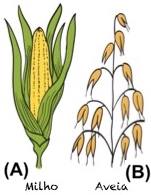
\includegraphics[width=1cm,height=1cm]{milho_aveia2.png} :
		\begin{itemize}
		\item $m=4$ Equações, logo, existirão 4 Variáveis Básicas (VB).
		\item $n=6$ Variáveis de decisão, logo, existirão $6-4$ ou $2$ Variáveis Não Básicas (VNB)
		\item Número de combinações será 
		$\frac{6!}{4!(6-4)!}=\frac{6 \cdot5 \cdot 4!}{4!2!}=\frac{30 \cdot \cancel{4!}}{\cancel{4!}2}=15$.
		\end{itemize}
	\end{itemize}
	}
\end{frame}